\documentclass[11pt,a4paper]{scrartcl}
\typearea{12}
\usepackage{graphicx}
\usepackage{pstricks}
\usepackage{listings}
\lstset{language=python}
\pagestyle{headings}
\markright{Computation Neuroscience - 3 the bucket equation}
\begin{document}

\subsection*{Introduction}
WORK IN PROGRESS - this is a half done DRAFT!\\ \\
These notes are about first order ordinary differential
equations. These equations appear frequently in neuroscience so it is
useful to consider them now before going any further.

\subsection*{Buckets of water}

In the simplest model of neurons their voltage dynamics is similar to
the dynamics of a bucket with a leak and the class of equations that
apply in this case will also be applied to synapses, for example.

\begin{center}
\setlength{\unitlength}{2mm}
\begin{picture}(20,40)
\linethickness{0.3mm}
\put(7,5){\line(1,0){8}}
\put(15,5){\line(0,1){20}}
\put(5,5){\line(0,1){20}}
\put(15,25){\line(-1,0){10}}
\put(6,5){\vector(0,-1){3}}
\put(10,27){\vector(0,-1){5}}
\put(17,10.5){\vector(0,-1){5.5}}
\put(17,14.5){\vector(0,1){5.5}}
\linethickness{0.075mm}
\put(5,20){\line(1,0){10}}
\put(7,2){$l(t)$}
\put(11,27){$i(t)$}
\put(16,12){$h(t)$}
\end{picture}
\end{center}

Consider a bucket, with straight sides which is filled to a height $h$
with water. Imagine the water leaks out of a hole in the bottom. The
rate the water leaks out depends on $h$; the larger $h$ is the larger
the pressure at the bottom is and hence the faster the water pours
out. In otherwords
\begin{equation}
l(t)\propto h(t)
\end{equation}
or 
\begin{equation}
l(t)= G h(t)
\end{equation}
where $G$ is a constant which will depend on the size of the hole and
complicated things like the viscosity of water. Of course, we are also
ignore lots of complicated stuff, like turbulence and so forth, but
since we are interested in the equation rather than the amount of
water in a bucket, this is fine. Imagine water also pours in the top
at a rate $i(t)$. This means the total rate of change of the amount of
water is $i(t)-Gh(t)$.

Now, $h(t)$ is the height of the water not the volume: the volume is
$Ch(t)$ where $C$ is the cross-sectional area of the bucket. The rate
of change of the volume is therefore
\begin{equation}
\frac{dCh(t)}{dt}=i(t)-Gh(t)
\end{equation}
or
\begin{equation}
\frac{dh}{dt}=\frac{1}{C}(i-Gh)
\end{equation}

Lets solve this equation for constant $i$ before going on to look at
neurons. Probably best to do this using an integrating factor, let
$\tau=C/G$ and $\tilde{\i}=i/G$
\begin{equation}
\tau\frac{dh}{dt}+h=\tilde{\i}
\end{equation}
then we multiply across by $\exp{t/tau}$
\begin{equation}
\tau e^{t/\tau}\frac{dh}{dt}+e^{t/\tau}h=\tilde{\i}e^{t/tau}
\end{equation}
Now we can rewrite the left hand side using the product rule
\begin{equation}
\frac{d}{dx}(uv)=u\frac{dv}{dx}+v\frac{du}{dx}
\end{equation}
to give
\begin{equation}
\tau\frac{d}{dt}\left(e^{t/\tau}h\right)=\tilde{\i}e^{t/tau}
\end{equation}
Now integrating both sides gives
\begin{equation}
e^{t/\tau}h=\tilde{\i}e^{t/tau}+A
\end{equation}
where $A$ is an integration constant. This gives
\begin{equation}
h=Ae^{-t/\tau}+\tilde{\i}
\end{equation}
and putting $t=0$ shows $A=h(0)-\tilde{\i}$ so
\begin{equation}
h(t)=[h(0)-\tilde{\i}]e^{-t/\tau}+\tilde{\i}
\end{equation}
so, basically, the value of $h$ decays exponentially until it
equilibriates with $\tilde{\i}$.

These dynamics make good intuitive sense; the more water there is in
the bucket, the higher the pressure will be at the leak and the
quicker the water will pour out. If there is just the right about of
water the rate the water pours out the leak will precisely match the
rate it pours in, this is the equilibrium. If there is more water than
required for equilibrium it will pour out faster than the flow coming
in, if there is less, it will pour out slower. Either way, as time
passes the height of the water will reach the equilibrium. The plot in
Fig.~\ref{bucket_v} illustrates this.

\begin{figure}
\begin{center}
% GNUPLOT: LaTeX picture with Postscript
\begingroup
  \makeatletter
  \providecommand\color[2][]{%
    \GenericError{(gnuplot) \space\space\space\@spaces}{%
      Package color not loaded in conjunction with
      terminal option `colourtext'%
    }{See the gnuplot documentation for explanation.%
    }{Either use 'blacktext' in gnuplot or load the package
      color.sty in LaTeX.}%
    \renewcommand\color[2][]{}%
  }%
  \providecommand\includegraphics[2][]{%
    \GenericError{(gnuplot) \space\space\space\@spaces}{%
      Package graphicx or graphics not loaded%
    }{See the gnuplot documentation for explanation.%
    }{The gnuplot epslatex terminal needs graphicx.sty or graphics.sty.}%
    \renewcommand\includegraphics[2][]{}%
  }%
  \providecommand\rotatebox[2]{#2}%
  \@ifundefined{ifGPcolor}{%
    \newif\ifGPcolor
    \GPcolorfalse
  }{}%
  \@ifundefined{ifGPblacktext}{%
    \newif\ifGPblacktext
    \GPblacktexttrue
  }{}%
  % define a \g@addto@macro without @ in the name:
  \let\gplgaddtomacro\g@addto@macro
  % define empty templates for all commands taking text:
  \gdef\gplbacktext{}%
  \gdef\gplfronttext{}%
  \makeatother
  \ifGPblacktext
    % no textcolor at all
    \def\colorrgb#1{}%
    \def\colorgray#1{}%
  \else
    % gray or color?
    \ifGPcolor
      \def\colorrgb#1{\color[rgb]{#1}}%
      \def\colorgray#1{\color[gray]{#1}}%
      \expandafter\def\csname LTw\endcsname{\color{white}}%
      \expandafter\def\csname LTb\endcsname{\color{black}}%
      \expandafter\def\csname LTa\endcsname{\color{black}}%
      \expandafter\def\csname LT0\endcsname{\color[rgb]{1,0,0}}%
      \expandafter\def\csname LT1\endcsname{\color[rgb]{0,1,0}}%
      \expandafter\def\csname LT2\endcsname{\color[rgb]{0,0,1}}%
      \expandafter\def\csname LT3\endcsname{\color[rgb]{1,0,1}}%
      \expandafter\def\csname LT4\endcsname{\color[rgb]{0,1,1}}%
      \expandafter\def\csname LT5\endcsname{\color[rgb]{1,1,0}}%
      \expandafter\def\csname LT6\endcsname{\color[rgb]{0,0,0}}%
      \expandafter\def\csname LT7\endcsname{\color[rgb]{1,0.3,0}}%
      \expandafter\def\csname LT8\endcsname{\color[rgb]{0.5,0.5,0.5}}%
    \else
      % gray
      \def\colorrgb#1{\color{black}}%
      \def\colorgray#1{\color[gray]{#1}}%
      \expandafter\def\csname LTw\endcsname{\color{white}}%
      \expandafter\def\csname LTb\endcsname{\color{black}}%
      \expandafter\def\csname LTa\endcsname{\color{black}}%
      \expandafter\def\csname LT0\endcsname{\color{black}}%
      \expandafter\def\csname LT1\endcsname{\color{black}}%
      \expandafter\def\csname LT2\endcsname{\color{black}}%
      \expandafter\def\csname LT3\endcsname{\color{black}}%
      \expandafter\def\csname LT4\endcsname{\color{black}}%
      \expandafter\def\csname LT5\endcsname{\color{black}}%
      \expandafter\def\csname LT6\endcsname{\color{black}}%
      \expandafter\def\csname LT7\endcsname{\color{black}}%
      \expandafter\def\csname LT8\endcsname{\color{black}}%
    \fi
  \fi
  \setlength{\unitlength}{0.0500bp}%
  \begin{picture}(5040.00,3528.00)%
    \gplgaddtomacro\gplbacktext{%
      \csname LTb\endcsname%
      \put(946,704){\makebox(0,0)[r]{\strut{} 0}}%
      \put(946,1131){\makebox(0,0)[r]{\strut{} 0.5}}%
      \put(946,1557){\makebox(0,0)[r]{\strut{} 1}}%
      \put(946,1984){\makebox(0,0)[r]{\strut{} 1.5}}%
      \put(946,2410){\makebox(0,0)[r]{\strut{} 2}}%
      \put(946,2837){\makebox(0,0)[r]{\strut{} 2.5}}%
      \put(946,3263){\makebox(0,0)[r]{\strut{} 3}}%
      \put(1078,484){\makebox(0,0){\strut{} 0}}%
      \put(1672,484){\makebox(0,0){\strut{} 0.5}}%
      \put(2266,484){\makebox(0,0){\strut{} 1}}%
      \put(2861,484){\makebox(0,0){\strut{} 1.5}}%
      \put(3455,484){\makebox(0,0){\strut{} 2}}%
      \put(4049,484){\makebox(0,0){\strut{} 2.5}}%
      \put(4643,484){\makebox(0,0){\strut{} 3}}%
      \put(176,1983){\rotatebox{-270}{\makebox(0,0){\strut{}$V(t)$}}}%
      \put(2860,154){\makebox(0,0){\strut{}$t$}}%
    }%
    \gplgaddtomacro\gplfronttext{%
      \csname LTb\endcsname%
      \put(3656,3090){\makebox(0,0)[r]{\strut{}$V(0)=2$}}%
      \csname LTb\endcsname%
      \put(3656,2870){\makebox(0,0)[r]{\strut{}$V(0)=3$}}%
      \csname LTb\endcsname%
      \put(3656,2650){\makebox(0,0)[r]{\strut{}$V(0)=0$}}%
    }%
    \gplbacktext
    \put(0,0){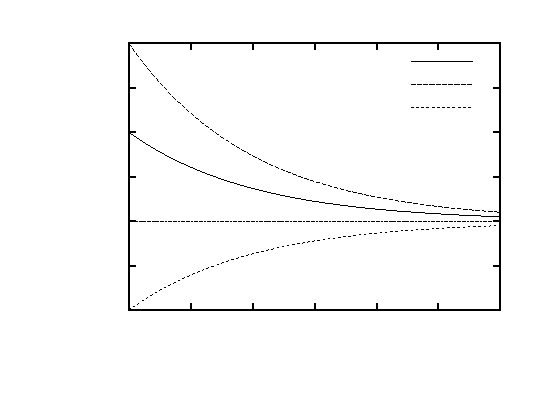
\includegraphics{bucket_v}}%
    \gplfronttext
  \end{picture}%
\endgroup

\end{center}
\caption{Exponential relaxation. The dynamics described by the
  \lq{}bucket equation\rq{} is very common. Here $V=[V(0)-I]\exp(-t/\tau)+I$ is plotted with $I=1$, $\tau=1$ and three different values of $V(0)$. $V(t)$ relaxes towards the equilibrium value $I=1$, the closer it gets, the slower it approaches.\label{bucket_v}}
\end{figure}

We have only discussed constant inputs; the variable input case is
harder and although it can sometimes be solved it is often easier just
to compute it numerically. This can be done either numerically, using
the Euler method or Runga-Kutta or approximating the variable input by
one that is constant for each discrete time step and then using the
solution for constant input. In any case, the effect is that the
solution kind of chases the input with a timescale set by $\tau$, that
is for very small $\tau$ is chases it quickly, so it is close to the
input, but for large $\tau$ it lags behind it and smooths it out. This
is sometimes described by saying that it \textsl{filters} the inout. There is an illustration in Fig.~\ref{chasing}.

\begin{figure}
\begin{center}
% GNUPLOT: LaTeX picture with Postscript
\begingroup
  \makeatletter
  \providecommand\color[2][]{%
    \GenericError{(gnuplot) \space\space\space\@spaces}{%
      Package color not loaded in conjunction with
      terminal option `colourtext'%
    }{See the gnuplot documentation for explanation.%
    }{Either use 'blacktext' in gnuplot or load the package
      color.sty in LaTeX.}%
    \renewcommand\color[2][]{}%
  }%
  \providecommand\includegraphics[2][]{%
    \GenericError{(gnuplot) \space\space\space\@spaces}{%
      Package graphicx or graphics not loaded%
    }{See the gnuplot documentation for explanation.%
    }{The gnuplot epslatex terminal needs graphicx.sty or graphics.sty.}%
    \renewcommand\includegraphics[2][]{}%
  }%
  \providecommand\rotatebox[2]{#2}%
  \@ifundefined{ifGPcolor}{%
    \newif\ifGPcolor
    \GPcolorfalse
  }{}%
  \@ifundefined{ifGPblacktext}{%
    \newif\ifGPblacktext
    \GPblacktexttrue
  }{}%
  % define a \g@addto@macro without @ in the name:
  \let\gplgaddtomacro\g@addto@macro
  % define empty templates for all commands taking text:
  \gdef\gplbacktext{}%
  \gdef\gplfronttext{}%
  \makeatother
  \ifGPblacktext
    % no textcolor at all
    \def\colorrgb#1{}%
    \def\colorgray#1{}%
  \else
    % gray or color?
    \ifGPcolor
      \def\colorrgb#1{\color[rgb]{#1}}%
      \def\colorgray#1{\color[gray]{#1}}%
      \expandafter\def\csname LTw\endcsname{\color{white}}%
      \expandafter\def\csname LTb\endcsname{\color{black}}%
      \expandafter\def\csname LTa\endcsname{\color{black}}%
      \expandafter\def\csname LT0\endcsname{\color[rgb]{1,0,0}}%
      \expandafter\def\csname LT1\endcsname{\color[rgb]{0,1,0}}%
      \expandafter\def\csname LT2\endcsname{\color[rgb]{0,0,1}}%
      \expandafter\def\csname LT3\endcsname{\color[rgb]{1,0,1}}%
      \expandafter\def\csname LT4\endcsname{\color[rgb]{0,1,1}}%
      \expandafter\def\csname LT5\endcsname{\color[rgb]{1,1,0}}%
      \expandafter\def\csname LT6\endcsname{\color[rgb]{0,0,0}}%
      \expandafter\def\csname LT7\endcsname{\color[rgb]{1,0.3,0}}%
      \expandafter\def\csname LT8\endcsname{\color[rgb]{0.5,0.5,0.5}}%
    \else
      % gray
      \def\colorrgb#1{\color{black}}%
      \def\colorgray#1{\color[gray]{#1}}%
      \expandafter\def\csname LTw\endcsname{\color{white}}%
      \expandafter\def\csname LTb\endcsname{\color{black}}%
      \expandafter\def\csname LTa\endcsname{\color{black}}%
      \expandafter\def\csname LT0\endcsname{\color{black}}%
      \expandafter\def\csname LT1\endcsname{\color{black}}%
      \expandafter\def\csname LT2\endcsname{\color{black}}%
      \expandafter\def\csname LT3\endcsname{\color{black}}%
      \expandafter\def\csname LT4\endcsname{\color{black}}%
      \expandafter\def\csname LT5\endcsname{\color{black}}%
      \expandafter\def\csname LT6\endcsname{\color{black}}%
      \expandafter\def\csname LT7\endcsname{\color{black}}%
      \expandafter\def\csname LT8\endcsname{\color{black}}%
    \fi
  \fi
  \setlength{\unitlength}{0.0500bp}%
  \begin{picture}(7200.00,5040.00)%
    \gplgaddtomacro\gplbacktext{%
      \csname LTb\endcsname%
      \put(726,440){\makebox(0,0)[r]{\strut{}-1}}%
      \put(726,873){\makebox(0,0)[r]{\strut{}-0.8}}%
      \put(726,1307){\makebox(0,0)[r]{\strut{}-0.6}}%
      \put(726,1740){\makebox(0,0)[r]{\strut{}-0.4}}%
      \put(726,2174){\makebox(0,0)[r]{\strut{}-0.2}}%
      \put(726,2608){\makebox(0,0)[r]{\strut{} 0}}%
      \put(726,3041){\makebox(0,0)[r]{\strut{} 0.2}}%
      \put(726,3475){\makebox(0,0)[r]{\strut{} 0.4}}%
      \put(726,3908){\makebox(0,0)[r]{\strut{} 0.6}}%
      \put(726,4342){\makebox(0,0)[r]{\strut{} 0.8}}%
      \put(726,4775){\makebox(0,0)[r]{\strut{} 1}}%
      \put(858,220){\makebox(0,0){\strut{} 0}}%
      \put(1453,220){\makebox(0,0){\strut{} 2}}%
      \put(2047,220){\makebox(0,0){\strut{} 4}}%
      \put(2642,220){\makebox(0,0){\strut{} 6}}%
      \put(3236,220){\makebox(0,0){\strut{} 8}}%
      \put(3831,220){\makebox(0,0){\strut{} 10}}%
      \put(4425,220){\makebox(0,0){\strut{} 12}}%
      \put(5020,220){\makebox(0,0){\strut{} 14}}%
      \put(5614,220){\makebox(0,0){\strut{} 16}}%
      \put(6209,220){\makebox(0,0){\strut{} 18}}%
      \put(6803,220){\makebox(0,0){\strut{} 20}}%
    }%
    \gplgaddtomacro\gplfronttext{%
      \csname LTb\endcsname%
      \put(5816,4602){\makebox(0,0)[r]{\strut{}$\tau=0.25$}}%
      \csname LTb\endcsname%
      \put(5816,4382){\makebox(0,0)[r]{\strut{}$\tau=2$}}%
      \csname LTb\endcsname%
      \put(5816,4162){\makebox(0,0)[r]{\strut{}$\tau=4$}}%
      \csname LTb\endcsname%
      \put(5816,3942){\makebox(0,0)[r]{\strut{}input}}%
    }%
    \gplbacktext
    \put(0,0){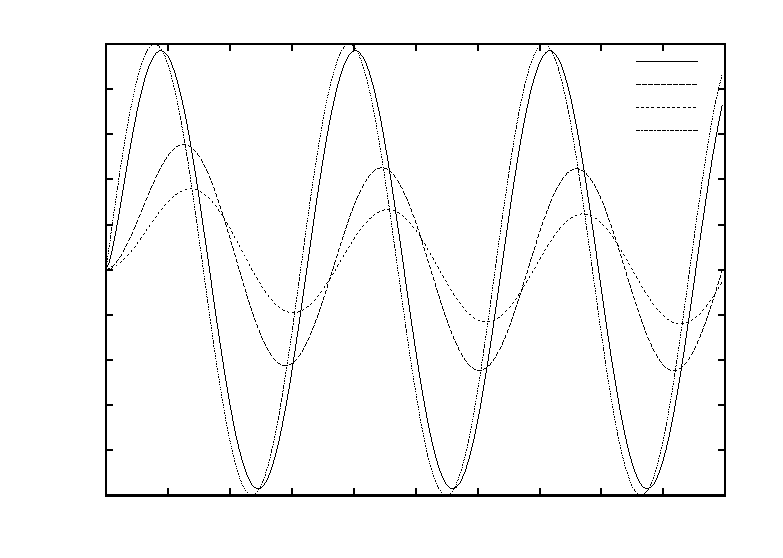
\includegraphics{chasing}}%
    \gplfronttext
  \end{picture}%
\endgroup

\end{center}
\caption{Variable input. Here the input is a sine wave $I=\sin{t}$ and the equation is evolved with $V(0)$ and three different $\tau$ values. For $\tau=0.25$ we see $V(t)$ closely matches the input whereas for larger $\tau$ it is smoother and lags behind.\label{chasing}}
\end{figure}


\end{document}

